\documentclass[tikz,border=2pt]{standalone}
\usepackage{amsmath}
\usetikzlibrary{arrows.meta}
\begin{document}
% M^B/M/1/K with K=10: a batch of 5 arrives when m=8 jobs are present.
% Complete acceptance admits 5 (8 <= K-1), partial acceptance admits K-m=2 and rejects 3,
% complete rejection rejects all 5 (8+5 > K).
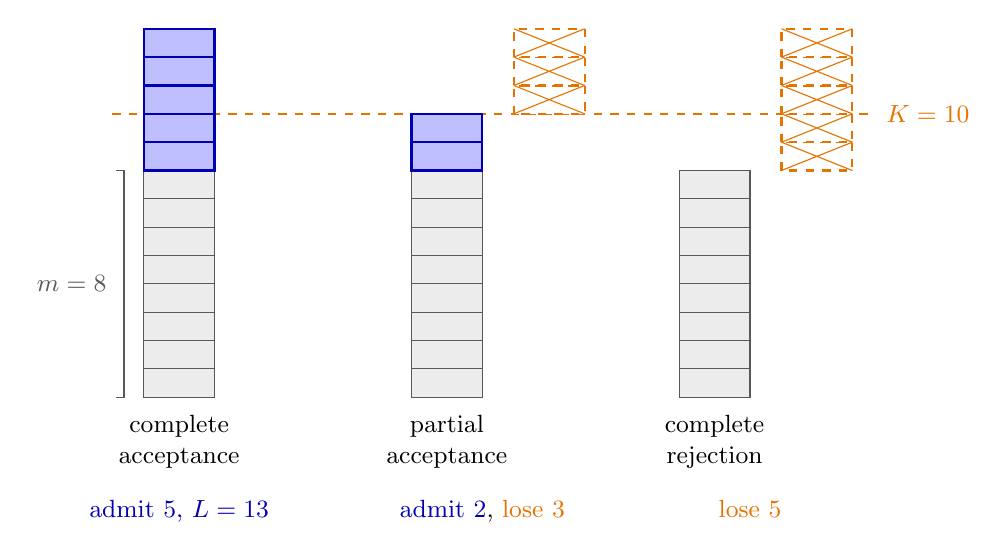
\begin{tikzpicture}[font=\small, >={Latex[length=2mm]}, x=1cm, y=0.36cm]
  \def\w{0.9}
  % capacity line (drawn first, so the boxes cover it)
  \draw[orange!90!black, thick, dashed] (-0.4,10) -- (9.3,10) node[right] {$K=10$};
  \foreach \c/\acc in {0/5, 1/2, 2/0} {
    \begin{scope}[xshift=\c*3.4cm]
      \foreach \j in {0,...,7} \draw[gray!70!black, fill=gray!15] (0,\j) rectangle (\w,\j+1);
      \foreach \j in {0,...,4} {
        \pgfmathtruncatemacro{\ok}{\j<\acc ? 1 : 0}
        \ifnum\ok=1
          \draw[blue!70!black, thick, fill=blue!25] (0,8+\j) rectangle (\w,9+\j);
        \else
          \draw[orange!90!black, thick, dashed, fill=white] (1.3,8+\j) rectangle (1.3+\w,9+\j);
          \draw[orange!90!black] (1.3,8+\j) -- (1.3+\w,9+\j) (1.3,9+\j) -- (1.3+\w,8+\j);
        \fi
      }
    \end{scope}
  }
  \node[anchor=north, align=center] at (0.45,-0.3) {complete\\acceptance};
  \node[anchor=north, align=center] at (3.85,-0.3) {partial\\acceptance};
  \node[anchor=north, align=center] at (7.25,-0.3) {complete\\rejection};
  \node[blue!70!black, anchor=north] at (0.45,-3.3) {admit $5$, $L=13$};
  \node[anchor=north] at (4.3,-3.3) {\textcolor{blue!70!black}{admit $2$}, \textcolor{orange!90!black}{lose $3$}};
  \node[orange!90!black, anchor=north] at (7.7,-3.3) {lose $5$};
  % present jobs
  \draw[gray!70!black] (-0.35,0) -- (-0.25,0) -- (-0.25,8) -- (-0.35,8);
  \node[gray!70!black, anchor=east] at (-0.35,4) {$m=8$};
\end{tikzpicture}
\end{document}
